\documentclass[10pt]{article}
\usepackage[margin=0.9in]{geometry}\usepackage[utf8]{inputenc}\usepackage[T1]{fontenc}\usepackage{lmodern}\usepackage{textcomp}
\usepackage{amsmath,amssymb}\usepackage{booktabs}\usepackage{graphicx}\usepackage[authoryear,round]{natbib}\usepackage{hyperref}\usepackage{xcolor}
\emergencystretch=2em\relax
\providecommand{\tightlist}{\setlength{\itemsep}{0pt}\setlength{\parskip}{0pt}}
\title{Five Raters Are Not a Distribution: What Learned Judges Can Learn from Human Disagreement, and Where to Spend the Annotation Budget}
\author{Anonymous}
\begin{document}\maketitle
\begin{abstract}
Learned judges are increasingly trained on the full histogram of human ratings rather than on a single label, with the stated aim of learning how people disagree. We ask what part of such a histogram a text-conditioned judge can learn. We separate two properties that prior work conflates: whether the histogram's shape beyond its location (mode and mean) is \emph{reproducible across raters}, and whether it is \emph{predictable from the text}. On rating panels from 14 datasets --- summarisation, offensiveness, politeness, helpfulness, sarcasm, valence, conversational safety, NLI, and seven software-engineering datasets including a 5,468-developer code-readability study --- a learner-free split-half analysis finds the shape beyond mode and mean poorly reproducible on every ordinal panel: its split-half reliability stays between 0.04 and 0.41 with 4--8 raters and below 0.3 even with 40 raters on the dense panels, so the raw histogram never forecasts a new rater better than its own mode and mean. A cross-fitted decoding analysis finds that the frozen representations of three model families recover at most a few percent of the reproducible ordinal shape (upper 95 \% bounds below 5 \% on seven of nine informative ordinal panels, at most 10.2 \% on all) but 17--26 \% of the NLI shape. Learned judges behave accordingly: statistic-preserving replacement of the shape of 70--83 \% of training targets leaves LoRA judges unchanged on two datasets, and alternative constructions of the per-item target change frozen-feature heads by at most a few thousandths of RPS in inconsistent directions, whereas discarding the distribution is worse on 9 of 11 panels. A rater--item decomposition shows that, beyond item location, rater-specific thresholds account for most held-out rating likelihood and no reproducible item-specific shape remains on the dense panels. At a fixed number of ratings, frozen-feature judges improve with more items rather than more raters per item on most panels, and end-to-end LoRA judges trained on one rating per item match those trained on seven (two base-model families) and beat judges trained on seven ratings for a seventh of the items; the marginal value of further ratings on covered items is task-dependent. We release per-dataset disagreement reliability cards and the estimators.
\end{abstract}

\section{Introduction}

Human raters disagree, and a growing line of work trains learned judges --- language models fine-tuned to score text --- on the full distribution of human ratings rather than on a single aggregated label (\citealp{chen2025beyond}; \citealp{singh2025distributions}; \citealp{kohli2026metric}; \citealp{benitosantos2025beyond}). The appeal is clear: a histogram records which neighbouring levels received mass and how concentrated the ratings were, and a judge that reproduces it would ``capture human disagreement'' rather than average it away. The data behind that appeal are thin. In most datasets the histogram is computed from three to nine people. Five ratings of a summary's coherence are a sample from a population of possible raters, and a model trained to reproduce the sample exactly is, in part, trained to reproduce sampling noise.

This paper asks a question that the literature on learning from label variation (\citealp{uma2021learning}; \citealp{plank2022problem}) has not asked in this form: \textbf{which part of a few-rater histogram can a text-conditioned judge learn?} We decompose every histogram into its \emph{location} (mode and mean) and the \emph{shape beyond location} (the residual allocation of mass once mode and mean are fixed), and we measure two properties of the shape that are usually conflated:

\begin{enumerate}
\def\labelenumi{\arabic{enumi}.}
\tightlist
\item
  \textbf{Reproducibility across raters.} If the same items were rated by a disjoint panel, would the shape come out the same? We estimate this learner-free with a split-half design: an exact identity, A1 = M $-$ 2X, relates the forecasting value of the raw histogram to the magnitude M of its residual relative to an exact mode-and-mean comparator and the cross-panel agreement X of that residual; the ratio $\rho$ = X/M is a split-half reliability of the shape at a given number of raters, and the raw histogram beats the comparator for predicting a new rater exactly when $\rho$ \textgreater{} $\tfrac12$.
\item
  \textbf{Predictability from the text.} Even a reproducible shape is useless to a judge unless the text carries it. We fit a cross-fitted ridge decoder from a frozen LLM's representation to the panel-1 residual and score it on an independent panel-2 residual with a proper-score gain G, reported also as the fraction G/X of the reproducible shape, against a within-cell feature-permutation control and a positive control.
\end{enumerate}

\textbf{Findings.} (i) \emph{The shape beyond mode and mean is poorly reproducible on ordinal scales.} Its split-half reliability is 0.04--0.41 on eight panels with 4--8 raters per item (intervals include 0 on four), and with three raters the mode-and-mean cell determines the histogram outright (\citet{crupi2025effectiveness}'s code-summary benchmark, MLCQ, Roy et al.). On the dense ordinal panels it stays below 0.3 up to 40 raters (Buse--Weimer 0.22, DICES 0.25 and 0.15, Dorn's Java panel 0.29), so on no ordinal panel does the raw histogram forecast a new rater better than its own mode and mean. ChaosNLI is the contrast: the NLI shape's reliability exceeds $\tfrac12$ from two to three raters and reaches 0.96--0.98 at 40. (ii) \emph{What is reproducible is mostly not in the text.} A cross-fitted linear decoder on frozen features, scored against an independent rater panel, recovers a fraction G/X of the reproducible shape whose upper 95 \% bound is 0.2--0.4 \% on SummEval, $\leq$ 0.4 \% on POPQUORN offensiveness, $\leq$ 2 \% on EmoBank, CSC and DICES-350, $\leq$ 4.6 \% on DICES-990, $\leq$ 5.4 \% on Dorn and $\leq$ 10.2 \% on HelpSteer2, consistently in Qwen2.5-7B, Qwen3-8B and OLMo-2-7B; on ChaosNLI MNLI it recovers 17--18 \% in all three families (intervals {[}0.11, 0.19{]}) and 26 \% on SNLI (Table 2). (iii) \emph{Learned judges do not use the shape.} Replacing the shape of 70--83 \% of training targets while preserving each target's exact mode and mean changes LoRA judges by $-$0.0001 {[}$-$0.0011, +0.0011{]} RPS on SummEval and +0.0000 {[}$-$0.0009, +0.0009{]} on POPQUORN, whereas destroying the location as well costs +0.012 and +0.003; the same intervention on ChaosNLI costs 0.016--0.052 KL. Across eleven ordinal panels and three feature families, training frozen-feature heads on the location-only comparator or on reliability-shrunk shapes changes held-out RPS by less than 0.001 with mixed signs; other smoothing constructions move it by up to $\pm$0.005 in panel-dependent directions; one-hot targets are worse on 9 of 11 panels. A user-held-out replication on POPQUORN, where no evaluator contributes to any target, gives the same signs. (iv) \emph{Beyond location, rating structure is mostly rater-side.} On the four panels with persistent rater identities, rater-specific cut-points improve held-out likelihood by 0.05--0.16 nats per rating while item-specific dispersion adds at most 0.012; on the dense panels no reproducible item-specific shape beyond mode and mean remains. This is consistent with --- though it does not by itself prove --- the reading that the shape a judge is asked to learn on rating scales is largely a property of who rated. (v) \emph{Budget.} At a fixed number of ratings, frozen-feature heads improve with more items rather than more raters per item on four of the five ordinal panels with more than 900 items and on both ChaosNLI panels (SummEval is flat; panels with $\leq$ 210 training items reverse). End-to-end LoRA judges trained on one rating per item match judges trained on all seven on SummEval (Qwen2.5, same batch, 3 seeds: $-$0.0027 {[}$-$0.0061, +0.0014{]}; OLMo-2: +0.0007 {[}$-$0.0056, +0.0069{]}) and beat judges trained on 144 $\times$ 7 by 0.023 / 0.0095 RPS; on POPQUORN a second rating per item recovers about two thirds of the single-rating gap. A prediction we registered --- that multi-rater items would pay off at fixed budget where the shape is text-predictable --- was falsified on ChaosNLI; we therefore do not derive the budget result from the mechanism and report the task-dependence of the marginal value of extra ratings as an observation.

\textbf{Contributions.} (1) Two reliabilities for disagreement --- across raters and across text --- with learner-free, cross-fitted estimators. (2) Disagreement reliability cards for every panel, telling a dataset builder whether the shape of disagreement is reproducible at the number of raters they can afford. (3) A rater--item decomposition of the ordinal structure beyond location. (4) Fixed-budget evidence, with frozen-feature heads in three model families and end-to-end LoRA judges, that covering items matters more than adding raters for training. Our earlier donor-replacement audit becomes the evidence that current training does not use the shape; shrinkage of the histogram survives as a tool for forecasting a new rater, not as a training method.

\textbf{What we do not claim.} That disagreement is noise (part of it is reproducible); that the text contains no residual information (we test linear decodability from three frozen model families); a theoretical rater-count threshold (a two-term 1/a model was falsified); a causal role of rater thresholds or of label structure in the ordinal--nominal difference; or a universal budget rule (\citet{zhang2021learning} find the opposite when a large single-label base already exists; see \S{}5).

\section{b. Related work}

\textbf{Learning from label variation.} Human label variation is increasingly treated as signal rather than noise (Aroyo \& Welty 2015; Pavlick \& Kwiatkowski 2019; \citealp{uma2021learning}; \citealp{plank2022problem}), and soft-label training is reported to improve calibration and robustness (\citealp{peterson2019human}; \citealp{collins2022eliciting}; \citealp{singh2025distributions}). For learned judges, \citet{chen2025beyond} train on human rating distributions; \citet{kohli2026metric} shows that on ChaosNLI the item-specific information in soft labels saturates around ten annotators for KL. These studies compare training targets; none separates the part of the histogram that is reproducible across raters from the part that is predictable from the input, which is the distinction our results turn on.

\textbf{Predicting disagreement.} Disagreement is partly predictable from text: NLI label distributions can be predicted to a degree (\citealp{zhou2022distributed}), reward models detect diverging preferences with AUROC around 0.6 (\citealp{zhang2025diverging}), and demographic information helps predict who disagrees (\citealp{wan2023everyone}). Our decoding analysis gives the matching quantity for the shape beyond mode and mean, normalised by its reproducible part, and finds the NLI and ordinal cases on opposite sides.

\textbf{Reliability of aggregates and rater effects.} Reliability of aggregated annotations depends on the number of raters (\citealp{wong2022krater}); rater severity and scale use are classical facets in many-facet Rasch measurement (\citealp{linacre1989mfrm}; \citealp{eckes2011mfrm}). We use the split-half logic and the rater facet, but apply them to the shape beyond location and connect them to what a text-conditioned judge can learn.

\textbf{Annotation budgets.} Whether to label more items or relabel existing ones is an old question in crowdsourcing (\citealp{sheng2008get}; \citealp{lin2014relabel}); for hard-label classifiers, labelling many items once is preferable above a worker-quality threshold (\citealp{khetan2018learning}). In NLP, \citet{zhang2021learning} find the opposite on ChaosNLI: replacing a few thousand single-label items by a few hundred ten-label items reduces KL --- in a regime where a large single-label base already exists and the evaluation targets the full distribution. Our budget results concern the complementary regime (every rating competes for items, ordinal quality ratings, judges trained only on the budgeted data), and on ChaosNLI we also observe a larger marginal value of a second rating than on ordinal panels; the two findings are consistent once the regime is stated.

\section{Two reliabilities of a disagreement histogram}
\begin{figure}[t]\centering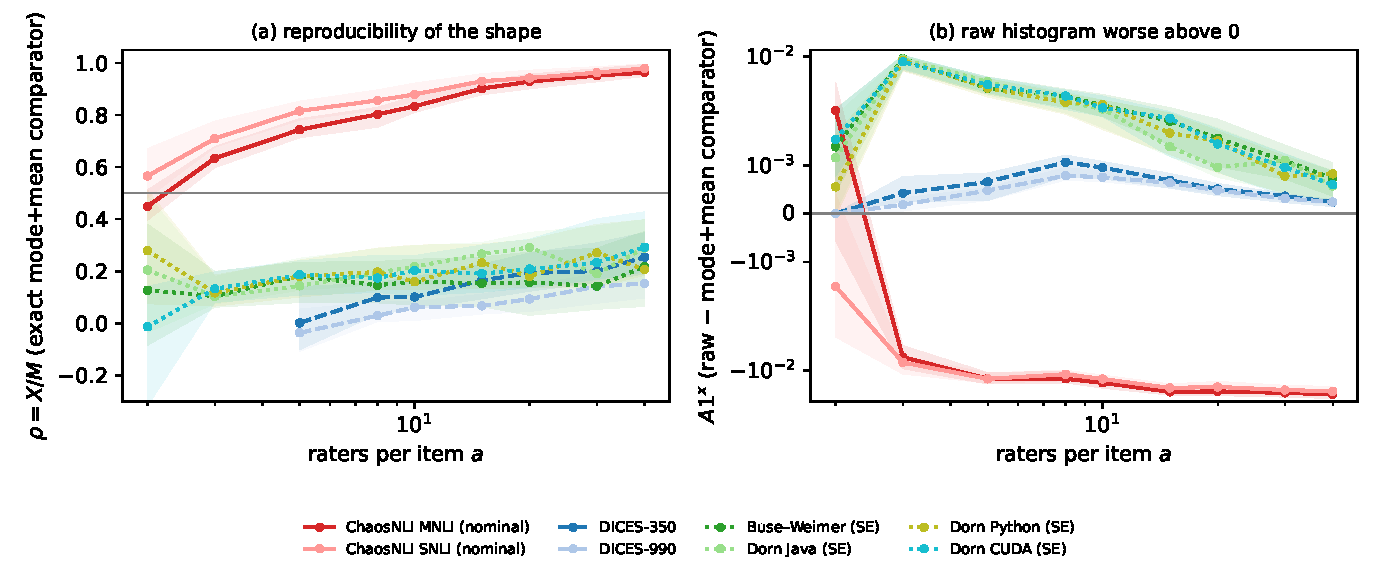
\includegraphics[width=\linewidth]{fig_reliability.pdf}\caption{Reliability of the shape beyond exact mode and mean against the number of raters per item, dense panels. (a) Split-half reliability $\rho=X/M$ relative to the exact mode-and-mean comparator, with 95\% item-cluster intervals; omitted where the residual is structurally empty or the ratio interval is wider than 1 (DICES with 2--5 ratings on a 3-level scale). The raw histogram beats the location-only forecast only above $\tfrac12$. (b) $A1^x$: positive means the raw histogram forecasts a new rater worse than its own mode and mean.}\label{fig:reliability}\end{figure}

\begin{table}[t]\centering\footnotesize
\caption{Disagreement reliability cards (exact mode-and-mean comparator). $\rho=X/M$: split-half reliability of the shape beyond mode and mean at $a$ raters, 95\% item-cluster interval; the raw histogram forecasts a new rater better than its own mode and mean only if $\rho>\tfrac12$ ($A1^x<0$). Support: share of items whose histogram can be changed at all with mode and mean fixed. Three-rater panels: the mode-and-mean cell determines the histogram (support 0). SE = software engineering.}\label{tab:cards}
\begin{tabular}{lrrlrr}\toprule panel & raters & $a$ & $\rho$ [95\% CI] & $A1^x$ & support \\\midrule
CSC sarcasm & 6 & 5 & 0.04 [-0.06, 0.13] & $+$0.0050 & 0.72 \\
EmoBank & 5 & 4 & 0.41 [0.27, 0.55] & $+$0.0003 & 0.14 \\
HelpSteer2 & 5 & 4 & 0.13 [0.04, 0.17] & $+$0.0036 & 0.45 \\
POPQUORN off. & 8 & 7 & 0.07 [-0.04, 0.25] & $+$0.0031 & 0.69 \\
POPQUORN pol. & 5 & 4 & 0.04 [-0.03, 0.12] & $+$0.0044 & 0.42 \\
Scalabrino$^{SE}$ & 9 & 8 & 0.19 [-0.24, 0.55] & $+$0.0027 & 0.69 \\
SummEval coh. & 8 & 7 & 0.35 [0.24, 0.48] & $+$0.0016 & 0.87 \\
SummEval rel. & 8 & 7 & 0.40 [0.30, 0.54] & $+$0.0008 & 0.79 \\
Buse--Weimer$^{SE}$ & 121 & 40 & 0.22 [0.06, 0.35] & $+$0.0007 & 0.89 \\
DICES-350 & 104 & 40 & 0.25 [0.19, 0.35] & $+$0.0002 & 1.00 \\
DICES-990 & 60 & 40 & 0.15 [0.10, 0.24] & $+$0.0002 & 1.00 \\
Dorn CUDA$^{SE}$ & 160 & 40 & 0.29 [0.20, 0.43] & $+$0.0006 & -- \\
Dorn Java$^{SE}$ & 160 & 40 & 0.29 [0.16, 0.40] & $+$0.0006 & -- \\
Dorn Python$^{SE}$ & 160 & 40 & 0.21 [0.18, 0.40] & $+$0.0008 & -- \\
ChaosNLI MNLI & 100 & 40 & 0.96 [0.95, 0.99] & $-$0.0186 & 1.00 \\
ChaosNLI SNLI & 100 & 40 & 0.98 [0.95, 1.00] & $-$0.0173 & 0.99 \\
Crupi CA$^{SE}$ & 3 & 2 & -- (no shape) & -- & 0.00 \\
Crupi conc.$^{SE}$ & 3 & 2 & -- (no shape) & -- & 0.00 \\
Crupi flu.$^{SE}$ & 3 & 2 & -- (no shape) & -- & 0.00 \\
MLCQ$^{SE}$ & 3 & 2 & -- (no shape) & -- & 0.00 \\
Roy CA$^{SE}$ & 3 & 2 & -- (no shape) & -- & 0.00 \\
\bottomrule\end{tabular}\end{table}

\textbf{Setting and notation.} Item \(i\) has ratings on \(K\) ordered levels from a panel of raters; the empirical histogram is \(h_i\). For ordinal scales we score forecasts with the ranked probability score, \(S(f,y)=\sum_k (F_f(k)-\mathbf 1[y\le k])^2/(K-1)\), and write \(C\) for the cumulative operator; for nominal tasks (ChaosNLI) \(S\) is the Brier score and \(C\) the identity. The \textbf{location} of a histogram is its exact mode and mean (nominal: modal class and modal mass); the \textbf{shape beyond location} is what remains once these are fixed. To isolate it we use the \emph{exact-T comparator} \(q_T\) of our earlier audit: a cross-fitted forecast built from other items in the same exact mode-and-mean cell (KL-projected onto the cell when the cell is sparse), so that \(q_T\) has the same mode and mean as \(h_i\) and differs from it only in shape. The residual of a histogram is \(r = C(h - q_T)\).

\subsection*{2.1 Reproducibility across raters (split-half reliability).} In each of \(R\) repetitions the ratings of every item are split at random into disjoint panels \(P_1\) (size \(a\)) and \(P_2\). Writing \(r_1 = C(h_1-q_T)\) and \(r_2 = C(h_2-q_T)\), with \(q_T\) computed from \(P_1\), the forecasting value of the raw histogram over the comparator obeys the exact identity \[A1 \;=\; \mathbb E\big[S(h_1,y)-S(q_T,y)\big]_{y\in P_2} \;=\; M - 2X,\qquad M=\|r_1\|^2/n,\; X=\langle r_1,r_2\rangle/n,\] so \(\rho = X/M\) is a split-half reliability of the shape and the raw histogram beats the location-only forecast exactly when \(\rho>\tfrac12\). \(M\) is the observed magnitude of the shape, \(X\) its agreement with an independent panel's shape; \(M-X\) is sampling noise. \(\rho\) is specific to the number of raters \(a\) and, as a ratio, unstable when \(M\) is tiny; we report it with intervals and omit it where the residual is structurally empty (e.g.~two or three ratings on a three-level scale). We also report the support of the donor-replacement intervention (the fraction of items whose histogram could be changed at all while preserving mode and mean). A smoother, response-based comparator that does not reproduce the noisy location gives larger values of \(\rho\) because it also credits location reliability; we use the exact comparator throughout. Intervals are item-cluster bootstraps in which all copies of a resampled item stay in one cross-fitting fold and the comparator is refitted in every replicate. Table 1 gives the resulting \emph{reliability cards}; Figure 1 traces \(\rho\) and \(A1^x\) against \(a\) on the dense panels.

\subsection*{2.2 Predictability from the text (decodability).} A judge sees the text, not the raters. Whether the reproducible shape is available to it is a separate question, which we answer with the representation the judges are built on: last-token hidden states of the frozen Qwen2.5-7B-Instruct (Qwen2.5-Coder for code panels) under the same rating prompt. A multi-output ridge decoder, group-cross-fitted over five item folds with a label-free PCA and a nested penalty, predicts \(r_1\) from the features; it is scored on the \emph{independent} panel \(r_2\) by the covariance \(V=\langle\hat r,r_2\rangle/n\) and by the proper-score gain \[G \;=\; \big(2\langle \hat r, r_2\rangle - \|\hat r\|^2\big)/n \;=\; \mathbb E_{y\in P_2}\big[S(q_T,y) - S(q_T + C^{-1}\hat r,\,y)\big],\] the exact reduction in score obtained by adding the decoded shape to the location-only forecast. Two controls accompany every estimate: a \emph{within-cell permutation} of the features among items with the same exact mode and mean (which must drive \(G\) to zero or below), and a \emph{positive control} that predicts the panel-1 mean with the same pipeline (which must be clearly positive, else the representation or the alignment is broken). Directions are symmetrised (\(P_1\leftrightarrow P_2\)) and bootstrapped over item clusters. Because a single layer is a weak probe, we repeat the analysis with per-layer mean- and last-token features and greedy selection of the best layers (the probing recipe of \citealp{li2026rethinking}).

\subsection*{2.3 Why the two can come apart.} \(\rho\) asks whether the shape is a property of the item's \emph{rater population}; \(G\) asks whether it is a property of the item's \emph{text}. A shape can be reproducible yet invisible to text --- for instance when it is produced by how particular kinds of raters use the scale --- and a text-predictable shape can be unreliable with few raters. Section 4 shows that the first case is the ordinal norm. Nothing in \S{}2.1 or \S{}2.2 trains a judge; both are measurements of the data and the representation, and both are released with the reliability cards so that a dataset builder can compute them before deciding how many raters to pay for.

\section{What learned judges use: the audit, condensed}

If a judge learned the shape beyond location, destroying that shape in its training targets would hurt it. Our donor-replacement audit (Sections 2--4 of the previous version; Tables T2b, T3b, T3c, T5) does exactly this with certified dose: for 70--83 \% of training items the histogram is replaced by another item's histogram projected onto the recipient's exact mode and mean (mean TV 0.30--0.35 among changed items), under two learners. \textbf{End-to-end LoRA judges} (Qwen2.5-7B-Instruct, the distributional objective of \citealp{chen2025beyond}; three optimizer--assignment realisations $\times$ three held-out-rater folds) change by $-$0.0001 {[}$-$0.0011, +0.0011{]} RPS on SummEval coherence and +0.0000 {[}$-$0.0009, +0.0009{]} on POPQUORN offensiveness, whereas destroying the location as well (mode-only replacement) costs +0.0120 {[}+0.0086, +0.0155{]} and +0.0029 {[}+0.0009, +0.0050{]} with every seed-by-fold cell positive. \textbf{Frozen-feature heads} on ten ordinal panels move by $-$0.0024 to +0.0006. On the nominal ChaosNLI panels the same kind of intervention --- scrambling the allocation of mass beyond the modal class while preserving the modal mass --- raises test KL by 0.016--0.052 at every annotation count.

A stronger version of the same test asks whether \emph{any} construction of the per-item target helps. We trained the heads on eleven ordinal panels with the raw histogram, the location-only comparator, reliability-shrunk shapes and locations, Dirichlet smoothing toward the mode prototype, label smoothing toward uniform and toward the marginal, and a cross-item smoothed comparator, thirty configurations each. No construction changes held-out RPS by more than $\pm$0.0005 with a consistent sign across panels; the one-hot target costs +0.003 to +0.010 everywhere. The learner pools location across items on its own and is indifferent to the per-item shape --- exactly what \S{}2.2 predicts for a shape it cannot see. Learned judges on ordinal scales learn location and calibration; on NLI they also learn shape, because there the shape is in the text.

\section{Where the ordinal shape comes from: a rater--item decomposition}
\begin{table}[t]\centering\footnotesize
\caption{Decodability of the residual beyond exact mode and mean from frozen representations of three model families: proper-score gain $G$ on an independent rater panel (95\% item-cluster bootstrap); positive control in parentheses (Spearman of the decoded vs held-out mean).}\label{tab:decode}
\begin{tabular}{llll}\toprule panel & Qwen2.5-7B & Qwen3-8B & OLMo-2-7B \\\midrule
Buse--Weimer$^{SE}$ & $+$0.00003 (0.54) & -- & -- \\
CSC sarcasm & $-$0.00001 (0.44) & $-$0.00001 (0.51) & $-$0.00001 (0.52) \\
DICES-350 & $-$0.00000 (0.47) & -- & -- \\
DICES-990 & $-$0.00000 (0.71) & $-$0.00000 (0.72) & $-$0.00000 (0.75) \\
Dorn (all)$^{SE}$ & $+$0.00002 (0.67) & -- & -- \\
EmoBank & $+$0.00000 (0.48) & $+$0.00000 (0.48) & $+$0.00001 (0.49) \\
HelpSteer2 & $+$0.00000 (0.36) & $+$0.00001 (0.39) & $+$0.00000 (0.27) \\
JetBrains naming$^{SE}$ & $+$0.00002 (0.30) & -- & -- \\
POPQUORN off. & $-$0.00001 (0.65) & $-$0.00000 (0.65) & $-$0.00001 (0.68) \\
Scalabrino$^{SE}$ & $-$0.00006 (0.41) & -- & -- \\
SummEval coh. & $-$0.00000 (0.41) & $+$0.00000 (0.36) & $-$0.00000 (0.27) \\
SummEval rel. & $-$0.00000 (0.33) & -- & -- \\
ChaosNLI MNLI & $+$0.00315 (0.29) & $+$0.00340 (0.32) & $+$0.00330 (0.24) \\
ChaosNLI SNLI & $+$0.00426 (0.41) & -- & -- \\
\bottomrule\end{tabular}\end{table}

The split-half analysis says the few-rater shape is mostly noise but not entirely (X \textgreater{} 0 on every panel); the decoding analysis says the reproducible part is not in the text. What is it, then? We fit three ordered-probit models to the rating matrices of the panels with persistent rater identities (Buse--Weimer, DICES-350, Scalabrino, the SummEval experts) and location-plus-dispersion models to the position panels: \(Y^*_{ir} = \theta_i + \sigma_i\,\varepsilon_{ir}\) with cut-points \(c_{r}\); \textbf{M0} item location with common cut-points, \textbf{M1} adding rater-specific cut-points (harshness), \textbf{M2} adding item-specific dispersion \(\sigma_i\) (the inverse of IRT discrimination). Held-out log-likelihood over random cells, five folds, with the dispersion penalty chosen on held-out data.

Rater thresholds carry the structure: M1 improves held-out likelihood by +0.111 (BW), +0.146 (DICES-350), +0.156 (Scalabrino), +0.104 / +0.047 (SummEval coherence / relevance) nats per rating; item dispersion adds +0.001 to +0.012 and over-fits on every 5--8-rating panel. Simulating rating matrices from the fitted models and re-running the split-half analysis closes the loop: on the dense ordinal panels the observed exact-T residual reliability is X $\approx$ 0 (BW $-$0.0001, DICES-350 +0.00003, DICES-990 +0.00002) and every model reproduces it --- once mode and mean are fixed there is \textbf{no reproducible item-specific shape} on these panels at all. SummEval retains a small residual (X = +0.0018 / +0.0016) that neither thresholds nor one-dimensional dispersion reproduce, and it is precisely this residual that the decoder of \S{}2.2 cannot read from the text. The mechanism is the textbook one of many-facet Rasch measurement (\citealp{linacre1989mfrm}; \citealp{eckes2011mfrm}), and we present it as measurement, not as a claim about raters' psychology; its consequence for judges is new: on ordinal rating scales the disagreement a text-conditioned model is asked to learn is largely a property of the people who rated, which no amount of text can supply without rater identity.

The annotation side confirms the same picture from a different angle. For forecasting a new rater from an item's own ratings, shrinking the \emph{location} toward the mode prototype by its split-half reliability improves RPS by $-$0.0048 {[}$-$0.0051, $-$0.0044{]} over the raw histogram (eight panels pooled), a cross-item smoothed comparator by $-$0.0113; shrinking the \emph{shape} by its reliability \(\lambda=X/M\) beats the raw histogram ($-$0.0021) but is indistinguishable from the location-only comparator ($-$0.0000 {[}$-$0.0000, $-$0.0000{]}) on every panel except SummEval, where \(\lambda\approx0.4\). What a few-rater histogram contributes beyond its location is, for practical purposes, nothing.

\section{Spending the annotation budget}
\begin{table}[t]\centering\footnotesize
\caption{End-to-end LoRA judges (distributional objective; Qwen2.5-7B and, for SummEval, OLMo-2-7B) at fixed rating budgets: test RPS minus the full-data judge, 95\% crossed bootstrap over optimizer seeds and test groups.}\label{tab:budget}
\begin{tabular}{llrrl}\toprule panel & design (items $\times$ ratings) & ratings & RPS & $-$ full data \\\midrule
SummEval (Qwen2.5, same batch, 3 seeds) & 960 $\times$ 1 & 960 & 0.1664 & $-$0.0027 [$-$0.0061, $+$0.0014] \\
SummEval (Qwen2.5, same batch, 3 seeds) & 480 $\times$ 2 & 960 & 0.1651 & $-$0.0040 [$-$0.0084, $-$0.0000] \\
SummEval (Qwen2.5, same batch, 3 seeds) & 144 $\times$ 7 & 1008 & 0.1897 & $+$0.0206 [$+$0.0163, $+$0.0247] \\
SummEval (Qwen2.5, same batch, 3 seeds) & 960 $\times$ 7 & 6720 & 0.1691 & -- \\
\midrule
POPQUORN (Qwen2.5) & 819 $\times$ 1 & 819 & 0.1294 & $+$0.0077 [$+$0.0046, $+$0.0110] \\
POPQUORN (Qwen2.5) & 117 $\times$ 7 & 819 & 0.1322 & $+$0.0105 [$+$0.0065, $+$0.0151] \\
POPQUORN (Qwen2.5) & 410 $\times$ 2 & 820 & 0.1339 & $+$0.0122 [$+$0.0083, $+$0.0167] \\
POPQUORN (Qwen2.5) & 205 $\times$ 4 & 820 & 0.1352 & $+$0.0135 [$+$0.0096, $+$0.0172] \\
POPQUORN (Qwen2.5) & 819 $\times$ 2 & 1638 & 0.1241 & $+$0.0024 [$+$0.0002, $+$0.0046] \\
POPQUORN (Qwen2.5) & 234 $\times$ 7 & 1638 & 0.1277 & $+$0.0061 [$+$0.0030, $+$0.0092] \\
POPQUORN (Qwen2.5) & 410 $\times$ 4 & 1640 & 0.1282 & $+$0.0065 [$+$0.0036, $+$0.0097] \\
POPQUORN (Qwen2.5) & 819 $\times$ 7 & 5733 & 0.1217 & -- \\
\midrule
SummEval (OLMo-2) & 960 $\times$ 1 & 960 & 0.1801 & $+$0.0007 [$-$0.0056, $+$0.0069] \\
SummEval (OLMo-2) & 480 $\times$ 2 & 960 & 0.1778 & $-$0.0016 [$-$0.0062, $+$0.0023] \\
SummEval (OLMo-2) & 144 $\times$ 7 & 1008 & 0.1896 & $+$0.0102 [$+$0.0049, $+$0.0156] \\
SummEval (OLMo-2) & 960 $\times$ 7 & 6720 & 0.1794 & -- \\
\bottomrule\end{tabular}\end{table}

If the shape is unlearnable and the location is what the judge learns, then every rating after the first on the same item buys at most a less noisy location, while a rating on a new item buys a new point for the regression the judge is implicitly fitting. We tested this directly by holding the total number of ratings fixed and trading items for raters.

\textbf{Frozen-feature heads} (nine ordinal panels, thirty configurations each; Table 5). On every panel with more than about 300 training items, more items with fewer ratings each wins monotonically: on DICES-990 at a budget of 594 ratings, 594 items $\times$ 1 rating gives RPS 0.203, 297 $\times$ 2 0.205, 148 $\times$ 4 0.207, 74 $\times$ 8 0.213 and 40 $\times$ 15 0.219; POPQUORN, HelpSteer2 and EmoBank follow the same order, SummEval is flat. The direction reverses only on small item sets (Buse--Weimer with 60 training items, DICES-350 with 210), where a single rating per item is too noisy a target. The same items-first order holds on ChaosNLI (959 $\times$ 1: KL 0.226; 30 $\times$ 32: 0.323) --- a result that falsified a prediction we had registered, namely that multi-rater items would pay off at fixed budget where the shape is text-predictable. They do not; where tasks differ is the \emph{marginal} value of a second rating on already-covered items (ChaosNLI $-$15 \%, ordinal heads $-$2 to $-$3 \%), which we report as an observation.

\textbf{End-to-end LoRA judges} (Table 6). On SummEval coherence, with the Chen et al. objective and the three held-out-expert folds of the audit, re-run in one batch with three optimizer seeds $\times$ three folds (SHRINKAGE\_PROTOCOL Amendment 6; results/lora\_budget\_v2/), a judge trained on 960 items $\times$ 1 randomly chosen rating (960 ratings) matches the judge trained on all 960 $\times$ 7 = 6,720 ratings ($-$0.0027 {[}$-$0.0061, +0.0014{]}, crossed bootstrap over seeds and test documents); 480 $\times$ 2 is equally good ($-$0.0040 {[}$-$0.0084, $-$0.0000{]}; vs 960 $\times$ 1: $-$0.0013 {[}$-$0.0073, +0.0039{]}), while 144 $\times$ 7 is worse than 960 $\times$ 1 by +0.0233 {[}+0.0176, +0.0285{]} --- both prespecified readings (``one rating per item matches the full data'', ``items first'') hold. An earlier two-seed block whose full-data reference came from a different batch had suggested that 960 $\times$ 1 \emph{beats} the full data ($-$0.0061); the same-batch re-run does not support that stronger claim. (The earlier block also gave 240 $\times$ 4: +0.0162 and 960 $\times$ 2: $-$0.0064 vs full; these designs were not re-run.) On POPQUORN offensiveness the ordering within each budget is again items-first (819 $\times$ 1 best at 820 ratings, 819 $\times$ 2 best at 1,638), but here extra ratings per item do help: 819 $\times$ 1 is +0.0077 {[}+0.0046, +0.0110{]} worse than the full 5,733-rating data and 819 $\times$ 2 recovers two thirds of that gap. The decisive part replicates on a non-Qwen base: with OLMo-2-7B on SummEval, 960 $\times$ 1 matches the full data (+0.0007 {[}$-$0.0056, +0.0069{]}) and 144 $\times$ 7 is worse than 960 $\times$ 1 by +0.0095 {[}+0.0020, +0.0157{]}; one versus two ratings per item is a tie on both bases. Single-rating training behaves like stochastic label sampling (\citealp{gheibi2026same}) and is consistent with the many-once-over-few-many results for hard-label classifiers (\citealp{khetan2018learning}; \citealp{lin2014relabel}); our contribution is the demonstration with distributional targets and end-to-end LLM judges, and the explanation of \S{}\S{}2--4 for why the raters' side of the budget buys so little.

\textbf{Rule.} For training a judge on an ordinal rating task, cover the items first; a second rating per item is worth between nothing (SummEval) and about half of the single-rating gap (POPQUORN), and further ratings less. Raters belong where a reliable reference distribution is itself the deliverable --- evaluation sets, and tasks such as NLI where the shape is in the text.

\section{Software-engineering panels}

Readability, summary quality and code-smell severity are rated on the same few-rater scales, and the same questions arise for code judges. Dorn's readability study (360 snippets in Java, Python and CUDA; 161--267 developers per snippet) gives the densest ordinal panel we know of; its reliability curve matches Buse--Weimer and DICES: the shape beyond mode and mean reaches a split-half reliability of only 0.2--0.3 even with 40 developers per snippet (Figure 1). The LLM-judge validation benchmarks of the field have three raters per item --- Crupi et al.'s code summaries, MLCQ's smell severities, Roy et al.'s summaries --- and with three raters the mode-and-mean cell determines the histogram: there is no shape to learn or to evaluate (support 0 \%). Scalabrino's nine-rater panel and JetBrains' 11--31-developer panel sit in between. Decoding from frozen features recovers none of it at a precision that matters: G/X is +0.03 {[}$-$0.03, +0.05{]} on Dorn's readability panel (360 snippets), $-$0.12 {[}$-$0.64, $-$0.01{]} on Scalabrino (a small over-fitting penalty on 124 snippets), and uninformative on Buse--Weimer (+0.07 {[}$-$0.07, +0.26{]}, 100 snippets) and JetBrains naming (+0.01 {[}$-$0.37, +0.03{]}, 120 identifiers) (results/decoding\_v2/). For SE human studies the practical reading is that three to five raters per artifact fix its location and nothing else, and that adding raters to a few artifacts does not make the shape of developer disagreement reproducible on these readability and quality scales.

\section{Limitations}

Base models: all frozen-feature results (decoding, target construction, fixed budget) replicate on Qwen3-8B and on the non-Qwen OLMo-2-7B (Table 2: ordinal G/X intervals include 0 on all six three-family panels with upper bounds $\leq$ 10 \%, ChaosNLI MNLI G/X 0.17 / 0.18 / 0.18 in Qwen2.5 / Qwen3 / OLMo-2; budget orderings within 0.002 RPS of each other; target constructions within $\pm$0.0005 except location-shrinking ones), and the end-to-end budget result replicates with an OLMo-2-7B LoRA judge on SummEval (the audit's LoRA blocks remain Qwen2.5-only); frozen-feature heads for breadth, end-to-end judges on two datasets; linear decoders --- we re-tested with per-layer features and greedy layer selection, not with non-linear or fine-tuned probes; SummEval's small unexplained residual; POPQUORN's position folds (a user-held-out check with real user ids, evaluators never in any target, confirms all four conclusions on offensiveness and politeness: mode+mean-preserving replacement $-$0.00004 / +0.00024, mode-only +0.0022 / +0.0029, one-hot +0.0042 / +0.0050, 4 ratings on a quarter of the items +0.0042 / +0.0030 worse than 1 rating on all); one registered prediction falsified and reported; effect sizes in the third decimal of RPS, to be read against the mode-only penalty of +0.012 and the budget effects of +0.02. We make no claim that disagreement is noise, that text contains no residual information, that a theoretical rater count exists, or that label structure causes the ordinal--nominal difference.

\bibliographystyle{plainnat}
\bibliography{../references}
\end{document}
